%%%%%%%%%%%%%%%%%%%%%%%%%%%%%%%%%%%%%%%%%%%%%%%%%%%%%%%%%%%%%%%%%%%%%%%%%%%%%%%%%%%%%%%%%%%%%%%%%%%%%%%%%%%%%%%%%
\documentclass[12pt]{article}
\usepackage{latexsym,epsfig,graphicx,epstopdf,amsmath,amssymb,amscd,pifont, multirow,chicago,psfrag,paralist,dsfont,url}
\usepackage[titletoc]{appendix}
%\usepackage{bm}

%%%%%%%%%%%%%%%%%%%%%%%%%%%%%%%%%%%%%%%%%%%%%%%%%%%%%%%%%%%%%%%%%%%%%%%%%%%%%%%%%%%%%%%%%%%%%%%%%%%%%%%%%%%%%%%%%
\textwidth  6.6in \textheight 9.2in \topmargin -.0in \oddsidemargin
-0.0in \evensidemargin -0.0in \pagestyle{plain}
\newcommand{\cmark}{\ding{51}}%
\newcommand{\xmark}{\ding{55}}%
\newcommand{\thetavec}{{\boldsymbol{\theta}}}
\newcommand{\veps}{\varepsilon}
\newcommand{\vepsvec}{{\boldsymbol{\varepsilon}}}
\newcommand{\Sigmavec}{{\boldsymbol{\Sigma}}}
\newcommand{\wvec}{{\boldsymbol{w}}}
\newcommand{\zerovec}{{\boldsymbol{0}}}
\newcommand{\onevec}{{\boldsymbol{1}}}
\newcommand{\Ivec}{{\boldsymbol{\rm I}}}
\newcommand{\betavec}{{\boldsymbol{\beta}}}
\newcommand{\betahat}{{\widehat{\beta}}}
\newcommand{\etavec}{{\boldsymbol{\eta}}}
\newcommand{\thetavecC}{{\boldsymbol{\theta}_C}}
\newcommand{\thetavecT}{{\boldsymbol{\theta}_T}}
\newcommand{\thetaveca}{\thetavec_{1}}
\newcommand{\thetavecb}{\thetavec_{2}}
\newcommand{\EE}{\mathbb{E}}
\newcommand{\Bset}{\mathbf{B}}
\newcommand{\Xset}{\mathbf{X}}
\newcommand{\Xmat}{\mathbf{X}}
\newcommand{\Pmat}{\mathbf{P}}
\newcommand{\pvec}{\boldsymbol{p}}
\newcommand{\Sset}{\mathbf{S}}
\newcommand{\cp}{{\rm CP}}
\newcommand{\pr}{{\rm Pr}}
\newcommand{\mvn}{{\rm MVN}}
\newcommand{\mse}{{\rm MSE}}
\newcommand{\emse}{{\rm EMSE}}
\newcommand{\TAE}{{\rm TAE}}
\newcommand{\MAE}{{\rm MAE}}
\newcommand{\bin}{{\rm bin}}
\newcommand{\enum}{{\rm enum}}
\newcommand{\Var}{{\rm Var}}
\newcommand{\muhat}{\widehat{\mu}}
\newcommand{\sigmahat}{\widehat{\sigma}}
\newcommand{\thetavechat}{\widehat{\thetavec}}
\newcommand{\thetavecmis}{\thetavec_{\ast}}
\newcommand{\mumis}{\mu_{\ast}}
\newcommand{\sigmamis}{\sigma_{\ast}}
\newcommand{\thetavecahat}{\widehat{\thetavec}_1}
\newcommand{\thetavecbhat}{\widehat{\thetavec}_2}
\newcommand{\amse}{{\rm AMSE}}
\newcommand{\avar}{{\rm AVar}}
\newcommand{\abias}{{\rm ABias}}
\newcommand{\bias}{{\rm Bias}}
%\newcommand{\diag}{{\rm Diag}}
\newcommand{\Arg}{{\rm Arg}}
\newcommand{\Ber}{{\rm Ber}}
\newcommand{\atantwo}{{\rm atan2}}
\newcommand{\ivec}{{\boldsymbol{i}}}
\newcommand{\dgoto}{\overset{d}{\rightarrow}}
\newcommand{\Pgoto}{\overset{P}{\rightarrow}}
\newcommand{\asgoto}{\overset{a.s.}{\longrightarrow}}
\newcommand{\sev}{\textrm{sev}}
\newcommand{\nor}{\textrm{nor}}
\newcommand{\N}{\textrm{N}}
\newcommand{\diag}{\textrm{Diag}}
\newcommand{\PMD}{\textrm{PMD}}
\newcommand{\wh}{\widehat}
\newcommand{\sigmaR}{\sigma_{R}}
\newcommand{\muR}{\mu_{R}}
\newtheorem{result}{Result}



\newcommand{\Xvec}{\boldsymbol{X}}
\newcommand{\Zvec}{\boldsymbol{Z}}
\newcommand{\xvec}{\boldsymbol{x}}
\newcommand{\kvec}{\boldsymbol{k}}
\newcommand{\rvec}{\boldsymbol{r}}
\newcommand{\minitab}[2][l]{\begin{tabular}{#1}#2\end{tabular}}
\newcommand{\fft}{\textrm{FFT}}




%mu sigma vector
\newcommand{\Sig}{\boldsymbol{\Sigma}}
\newcommand{\mvec}{\boldsymbol{\mu}}

%methods
\newcommand{\SIM}{{\rm SIM}}
\newcommand{\NA}{{\rm NA}}
\newcommand{\dft}{{\rm DFT-CF}}



\newcommand{\qed}{\hfill\blacksquare}
\newcommand{\qedw}{\hfill \ensuremath{\Box}}


%%%%%%%%%%%%%%%%%%%%%%%%%%%%%%%%%%%%%%%%%%%%%%%%%%%%%%%%%%%%%%%%%%%%%%%%%%%%%%%%%%%%%%%%%%%%%%%%%%%%%%%%%%%%%%%%%
\def\baselinestretch{1.25}
\renewcommand{\arraystretch}{.8}
%%%%%%%%%%%%%%%%%%%%%%%%%%%%%%%%%%%%%%%%%%%%%%%%%%%%%%%%%%%%%%%%%%%%%%%%%%%%%%%%%%%%%%%%%%%%%%%%%%%%%%%%%%%%%%%%%

\usepackage[ruled,vlined]{algorithm2e}
%%%%%%%%%%%%%%%%%%%%%%%%%%%%%%%%%%%%%%%%%%%%%%%%%%%%%%%%%%%%%%%%%%%%%%%%%%%%%%%%%%%%%%%%%%%%%%%%%%%%%%%%%%%%%%%%%

%\theoremstyle{definition}
%\newtheorem{exmp}{Example}[section]



\newtheorem{example}{Example}
\newtheorem{thm}{Theorem}
\newtheorem{ppt}{Property}
\newtheorem{lemma}{Lemma}
\newtheorem{remark}{Remark}
\newtheorem{defn}{Definition}
\newtheorem{corl}{Corollary}



%%%%%%%%%%%%%%%%%%%%%%%%%%%%%%%%%%%%%%%%%%%%%%%%%%%%%%%%%%%%%%%%%%%%%%%%%%%%%%%%%%%%%%%%%%%%%%%%%%%%%%%%%%%%%%%%%
\textwidth  6.6in \textheight 9.2in \topmargin -.5in \oddsidemargin
-0.0in \evensidemargin -0.0in \pagestyle{plain}

%%%%%%%%%%%%%%%%%%%%%%%%%%%%%%%%%%%%%%%%%%%%%%%%%%%%%%%%%%%%%%%%%%%%%%%%%%%%%%%%%%%%%%%%%%%%%%%%%%%%%%%%%%%%%%%%%
\def\baselinestretch{1.25}
\renewcommand{\arraystretch}{.8}
%%%%%%%%%%%%%%%%%%%%%%%%%%%%%%%%%%%%%%%%%%%%%%%%%%%%%%%%%%%%%%%%%%%%%%%%%%%%%%%%%%%%%%%%%%%%%%%%%%%%%%%%%%%%%%%%%

\setcounter{tocdepth}{2}

%-------------------------------------------------------------------------
\begin{document}
%%%%%%%%%%%%TITLE%%%%%%%%%%%%%%%%%%%%%%%%%%%%%%%%%%%

%\title{The Computing of Probability Mass Functions for the Poisson Multinomial Distribution}

\title{The Poisson Multinomial Distribution and Its Applications in Voting Theory, Ecological Inference, and Machine Learning}


%\iffalse
\author{
Zhengzhi Lin, Yueyao Wang, and Yili Hong\\[1.5ex]
{Department of Statistics, Virginia Tech, Blacksburg, VA 24061}
}
%\fi
	
\date{\today}
	
\maketitle
	%%%%%%%%%%%%%%%%%%%%%%%%%%%%%%%%%%%%%%%%%%%%%%%%%%%%%%%%%%%%%%%%%%%%%%%%%%%%%%%%%%%%%%%%%%%%%%%%%%%%%%%%%%%%%%%%
\begin{abstract}
The Poisson Multinomial Distribution (PMD) is the sum of $n$ independent indicators, in which each indicator is an $m$ element vector that follows a multinomial distribution. The PMD is useful in many areas such as, machine learning, uncertainty quantification, and voting theory. The distribution function (e.g., the probability mass function) has been studied by many authors for a long time, but there is no general computing method available for its distribution functions. In this paper, we develop algorithms to compute the probability mass function for the PMD, and we develop an R package that can calculate the probability mass function efficiently. We also study the accuracy of different methods. We illustrate the use of the PMD with three applications from voting theory, ecological inference, machine learning. We also provide examples to demonstrate the use of the R package.
		
\textbf{Key Words:} Binomial distribution; Classification; Poisson Binomial Distribution; Machine Learning; Uncertainty Quantification;  Voting Theory
\end{abstract}
	
	%%%%%%%%%%%%%%%%%%%%%%%%%%%%%%%%%%%%%%%%%%%%%%%%%%%%%%%%%%%%%%%%%%%%%%%%%%%%%%%%%%%%%%%%%%%%%%%%%%%%%%%%%%%%%%%%%%%%%
\newpage
\tableofcontents
\newpage
	
	%%%%%%%%%%%%%%%%%%%%%%%%%%%%%%%%%%%%%%%%%%%%%%%%%%%%%%%%%%%%%%%%%%%%%%%%%%%%%%%%%%%%%%%%%%%%%%%%%%%%%%%%%%%%%%%%%%%%%
\section{Introduction}
\subsection{Motivation}

The Poisson Multinomial Distribution ($\PMD$) is defined as sum of different independent Multinomial distributions. It has applications in game theory (\citeNP{Cheng2017PlayingAG}), digital imaging (\citeNP{akter2019double}), machine learning (\citeNP{kamath2014learning}), etc. One intriguing area that involves $\PMD$ is political science. It would be good to illustrate $\PMD$ a little bit further via a very simple example in election scenario. Suppose a committee with $\rm n$  independent members needs to elect a chairman between $\rm m$ candidates. Each member has a different voting behavior. Mostly, people pay attention to the result of an election. Statisticians focus on the probability for each electoral outcome to happen. An $\rm (n,m)$ $\PMD$ is a perfect model for this example by seeing members as independent random variables following different Multinomial distributions. The probability vector of the Multinomial distribution regards to the probabilities for a member voting for each candidates. By this way, we will be allowed to compute the probability of each electoral result which is referred as probability mass function of $\PMD$. Without a doubt, computing the probabilities of electoral results will be of greatest concern. Enumeration could be a fine method when $\rm n \times m$ is small. However, when we have more members(large $\rm n$) or more candidates(large $\rm m$), the computing will be a dilemma that is impossible to overcome by enumeration. Thus arises the need of methods that are computationally cheap and precise at the meantime. Additionally, in machine learning, especially in classification context, when we classify $\rm n$ samples one by one into $\rm m$ categories, then the total number of samples assigned to each category follows a $\PMD$. People who study the probability of classification outcomes also encounters same dilemma. Not only in the field of classification and political science, computing pmf is frequently required in scenarios that $\PMD$s are involved. However, there is no existing algorithm for computing pmf for PMD. Hereby it is a necessity to build one that can calculate pmf of $\PMD$s efficiently.



\subsection{Related Literature and Contribution of This Work}

%Ecological inference https://www.pnas.org/content/96/19/10578


Some former studies have uncover $\PMD$'s structure and properties, \citeN{diakonikolas2016fourier} shows the Fourier transformation of $\PMD$ is sparse and provide a theorem that there exist algorithms to calculate PMD's density. \citeN{Daskalakis2015OnTS} also prove us PMD is $\epsilon$-cover and Central Limit Theory is valid for PMD. Other papers such as \citeN{akter2019double} illustrates us some interesting applications of PMD and its sparsity property. Motivated by the huge practical value of $\PMD$, we develop an algorithm based on prior studies to compute probability mass function of $\PMD$s. Our algorithm contains three methods. They are $\dft$ which is based on multi-dimensional Fourier transformation, $\SIM$ that is a simulation method and $\NA$ which applies ${\rm C.L.T}$ to approximate the $\PMD$. The algorithm enables researchers to calculate pmf of $\PMD$s under certain requirements of accuracy and timing even when $\rm n$ and $\rm m$ gets large. We also construct a R package to perform our algorithm, the functions contained in the package are able to compute pmf and cdf of $\PMD$ using all methods we mentioned in this paper as well as generate random samples from given $\PMD$.





\subsection{Overview}
The rest of the paper is organized as follows. In the second part, we describe the mathematical definition of Poisson Multinomial distribution and list some of its useful properties. In the third part, we introduce three methods that we include in the algorithm to compute $\PMD$s' pmf by details. The fourth part of this article studies the accuracy and time efficiency characteristics of the three methods. In the fifth part, we illustrate application of our algorithm via three examples respectively in the fields of voting theory, statistical inference for aggregated data and classification. In the sixth part, we introduce our R package that implemented with the algorithm and the seventh part of this paper draws the conclusion and prospective research areas.




%%%%%%%%%%%%%%%%%%%%%%%%%%%%%%%%%%%%%%%%%%%%%%%
\section{Poisson Multinomial Distribution}
%%%%%%%%%%%%%%%%%%%%%%%%%%%%%%%%%%%%%%%%%%%%%%%%%%%%%%%%%%%%%%%%%%%%%%%%%%%%%%%%%%
\subsection{Definition of the Distribution}

Let $\Ivec_{i} = (I_{i1}, \dots, I_{im})', i=1, \dots, n$ be a random indicator vector that follows multinomial distribution with associated probabilities $\pvec_{i} = (p_{i1}, \dots, p_{im})'$ and for a fixed $i$, $\sum_{j=1}^{m} I_{ij}=1$. Then the sum $\Xvec = (X_{1}, \dots, X_{m})'= \sum_{i=1}^{n}\Ivec_{i}$ follows a Poisson Multinomial Distribution with corresponding probability matrix $\Pmat_{\rm n \times m} = (\pvec_{1}, \dots, \pvec_{n})'$, denoted it as
$$\Xvec \sim \PMD(\Pmat_{\rm n\times m}).$$ where $X_{j} = \sum_{i=1}^{n} I_{ij}, j=1,\dots,m$. The matrix $\Pmat$ is called Success Probability Matrix (SPM).

\begin{equation*}
\Pmat_{\rm n \times m} = \begin{pmatrix}
p_{11} &  \dots & p_{1m} \\
\vdots & \ddots & \vdots \\
p_{n1} &  \dots & p_{nm} \\
\end{pmatrix}.
\end{equation*}
It is trivial to find that the random variables, $X_1, \dots, X_{m}$ actually have to be constrained under linear equation $$\sum_{j=1}^{m}X_{j} = n$$. Hence we can replace one of them, for instance, $X_m$ with $n-\sum_{j=1}^{m-1}X_j$.

Let vector $\xvec = (x_1,\dots,x_m)'$ be a realization of a $\PMD$ random variable $\Xmat$, the probability mass function (pmf) of PMD,
$$\text{Pr}(\Xmat=\xvec) = \text{Pr} \left( X_1 = x_1, \dots, X_m = x_{m-1}, X_{m} = n-\sum_{i=1}^{m}x_i \right)$$
is of interest. 

\begin{example}\normalfont
Suppose there are three candidates and four voters, the result of voting is a random variable $\Xmat \sim \PMD(\Pmat)$. Based on prior information,
\begin{equation*}
\Pmat_{4 \times 3} = \begin{pmatrix}
0.1 &  0.2 & 0.7\\
0.5 & 0.2 & 0.3\\
0.4 &  0.5 & 0.1\\
0.8 & 0.1 & 0.1
\end{pmatrix}.
\end{equation*}
There are 15 distinct outcomes of the election, that is, the pmf is composed of 15 distinct non-zero mass points. It is trivial to compute the pmf of $\Xmat$ through enumeration. For instance, the probability of a result that the first candidate gets 4 votes and others gets 0 vote, that is, $\xvec =  (4,0,0)'$.
\begin{equation*}
P\{\Xmat = \xvec \} = 0.1\times 0.5 \times 0.4 \times 0.8 = 0.016.
\end{equation*}
Also, the probability of $\Xmat=(1,3,0)'$ is
\begin{align*}
P\{\Xmat = (1,3,0)\}  =  & 0.1\times 0.2 \times 0.5 \times 0.1 +
 0.5\times0.2\times0.5 \times 0.1 \\
 & + 0.4\times0.2\times0.2\times0.1 + 0.8\times0.2\times0.2\times0.5 = 0.0236.
\end{align*}
\qedw
\end{example}

When dimension of $\Pmat$ is small, enumeration is an exact way to calculate the probability mass function. However, as $\rm n \times m$ gets larger enumeration becomes impossible since we will have to compute $\binom{n+m-1}{m-1}$ possible outcomes which is calculated by the number of non-negtive integer solution for equation $x_1 + \dots + x_m = n$.


Note that when the SPM is identical across all rows, that is, $\rm I_{i}$, $i = 1, \dots n$ are identically distributed, the distribution of $X$ can be simplified as multinomial distribution. Hence, the $\PMD$ is a generalization of the multinomial distribution. When $m=1$, the $\PMD$ is reduced to the Poisson binomial distribution as in \citeN{hong2013computing}.

In related literature, \citeN{hong2013computing} consider the exact and approximate methods for computing the pmf of the Poisson binomial distribution. \citeN{zhang2018generalized} introduce the general Poisson binomial distribution and develop an algorithm to compute its distribution functions.

Now let's take a look of some basic properties of Poisson Multinomial Distributions.

\subsection{Properties of the Distribution}
\begin{ppt}\normalfont
Given random variable $\Xmat$ that follows a Poisson Multinomial distribution with $\Pmat_{\rm n\times m}$, the mean of $\Xmat$ is
   $$\\E(\Xmat) = \boldsymbol{\mu} = \left( p_{\cdot1} ,\dots,p_{\cdot,m-1},p_{\cdot m}\right)'$$ where $p_{\cdot k} = \sum_{i=1}^{n}p_{i k}$.\\
The variance-covariance matrix of $\Xmat$ is an $m \times m$ matrix $\Sig$ that has entries $\Sigma_{ij},i=1,\dots,m,j=1,\dots,m$ defined as
\begin{equation*}
   \Sigma_{ij} =
           \begin{cases}
             \sum_{k=1}^{n}p_{ki}(1-p_{ki}) & \quad \text{if } i=j\\
             -\sum_{k=1}^{n}p_{ki}p_{kj} & \quad \text{if } i \neq j\\
           \end{cases}
\end{equation*}\\
The CF for the $\PMD$ is
\begin{equation*}
\phi_{\Xmat}(t_1, \dots, t_{m-1}) = \phi_{(X_1,\dots,X_m)'}(t_1, \dots, t_{m-1})  =  \sum_{x_1 = 0}^{n} \cdots \sum_{x_{m-1} = 0}^n p(x_1,\ldots,x_{m-1})\exp\left(\ivec\sum_{j=1}^{m-1}t_jx_j\right).
\end{equation*}
where  $\ivec=\sqrt{-1}$.
\qedw
\end{ppt}
The derivations of mean and characteristic function are as trivial as following the definitions. The $\Sig$ can be calculated by observing that for any fix $i=1,\dots,n$, $I_{ij}$ and $I_{ik}$ has covariance $-p_{ij}p_{ik},j=1,\dots,m,k=1,\dots,m$. One important thing is that the covariance matrix $\Sig$ is singular because the elements of $\Xvec$ are linear dependent.

Let $\Xvec^{\star}=(X_1,\dots,X_{m-1})'$ with corresponding $\Pmat^{\star}$ equals to the first $m-1$ columns of $\Pmat$, then it has a non-singular $(m-1) \times (m-1)$ covariance matrix $\boldsymbol{\Sigma}_{0}$. Similar to $\Sig$, the covariance matrix
 $$\Var(\Xvec^{\star}) =\Sig^{\star}=\sum_{i=1}^n[\diag(\pvec_i)-\pvec_i\pvec_i']$$
where $\pvec_i$ is the $i$th row of $\Pmat^{\star}$. Also,  
  $$\EE(\Xvec^{\star}) =\boldsymbol{\mu^{\star}} = \left( p_{\cdot1} ,\dots,p_{\cdot,m-1}\right)'$$
 We call $\Xvec^{\star}$ a reduced $\PMD$ of $\Xvec$ and $\Pmat^{\star}$ a reduced SPM of $\Pmat$. Respectively, $\Sig^{\star}$ is the reduced covariance matrix of $\Sig$ and $\mvec^{\star}$.
\begin{ppt}\normalfont
If the SPM $\Pmat$ can be written as a combination of diagonal matrices $\Pmat_1, \Pmat_2, \dots, \Pmat_{K}$, $\Pmat = \diag(\Pmat_{\rm k}), k=1,\dots,K$. Then the outcome of $\Pmat$, $\boldsymbol{x}$ can hereby be decomposed in to outcomes of the diagonal matrices, $\xvec= (\xvec_{1},\dots,\xvec_{\rm K})$.  There will also have random variables $\Xvec_{\rm i} \sim \PMD(\Pmat_{\rm i})$, respectively. The pmf can computed as the product of the corresponding marginal pmfs. That is
\begin{align*}
\rm Pr(\Xvec=\xvec)= \rm \Pr(\Xvec_{1}=\xvec_{1}, \dots, \Xvec_{\rm K}=\xvec_{\rm K})= \prod_{k=1}^K \rm Pr(\Xvec_{k} = \xvec_{k}).
\end{align*}
\qedw
\end{ppt}

To show this, we assume $\Pmat$ is $\rm n \times m$ and $\Pmat_{\rm k}$ is $n_k \times m_k$. $\sum_{k=1}^K n_k = n$ and $\sum_{k=1}^K m_k = m$. Suppose there are $n$ voters to vote $m$ candidates, certain groups of voters only vote for certain groups of candidates and there are no overlaps . Heuristically, we can separate candidates and voters into independent groups, in each group $k$, $k = 1,\dots,K$, voters voting for corresponding candidates described by probability matrix $\Pmat_{\rm k}$. Strict proof can be done by decomposition of characteristic function of $\Pmat$ into characteristic functions of $\Pmat_{\rm k}$'s.



\section{Computation of The Probability Mass Function}\label{sec:CA.driving.study}
%%%%%%%%%%%%%%%%%%%%%%%%%%%%%%%%%%%%%%%%%%%%%%%%%%%%%%%%%%%%%%%%%%%%%%%%%%%%%%%%%%%%
We introduce three methods for computing the pmf, which are the method based on multidimensional discrete Fourier transform ($\dft$), the normal approximation ($\NA$) method, and simulation based method($\SIM$). $\dft$ is an exact method while the other two are approximate methods.

%%%%%%%%%%%%%%%%%%%%%%%%%%%%%%%%%%%%%%%%%%%%%%%%%%%%%%%%%%%%%%%%%%%%%%%%%%%%%%%%%%%%%%%%%%%%%%%%%%
\subsection{The $\dft$ Method}
%%%%%%%%%%%%%%%%%%%%%%%%%%%%%%%%%%%%%%%%%%%%%%%%%%%%%%%%%%%%%%%%%%%%%%%%%%%%%%%%%%%%%%%%%%%%%%%%%%
Although $\PMD$ is of great importance, its pmf is obscure and no straightforward form has been found so far. However, its characteristic function(cf) can be wrote down in an accessible form. The cf is just a Fourier transformation of pmf, thus we can obtain pmf via Fourier transformed cf. Notice the pmf is discrete, so the discrete Fourier transformation will be used. In this section we provide an exact method to compute the pmf of the PMD using multidimensional discrete Fourier transformation. To speed up the computing, we implement Fast Fourier Transformation algorithm($\fft$). %fft reference

Suppose a random variable $\Xvec =  (X_1, \dots, X_{m})' \sim \PMD(\Pmat)$, where $\Pmat = (p_{ij}), i=1,\dots,n,j=1,\dots,m$. Consider $\Xvec^{\star} = (X_1, \dots, X_{m-1})'$ will be equivalent since the last element of $\Xvec$ is redundant. The cf of $\Xvec^{\star}$ is 

\begin{align}
\phi(t_1, \dots, t_{m-1}) & = \EE\left[\exp\left(\ivec\sum_{j=1}^{m-1}t_jX_j\right)\right]=\EE\left[\exp\left(\ivec\sum_{i = 1}^n \sum_{j=1}^{m-1}t_j I_{ij}\right)\right].
\end{align}
Here $\ivec=\sqrt{-1}$. We notice
\begin{equation}
\begin{split}
  &\EE\left[\exp\left(\ivec\sum_{j=1}^{m-1}t_jX_j\right)\right] = \sum_{x_1 = 0}^{n}\cdots \sum_{x_{m-1} = 0}^n p(x_1,\ldots,x_{m-1})\exp\left(\ivec\sum_{j=1}^{m-1}t_jx_j\right).\\
\end{split}
\end{equation}
By definition, 
\begin{equation}
\exp\left(\ivec\sum_{j=1}^{m-1}t_jX_j\right)= \exp\left(\ivec\sum_{i = 1}^n \sum_{j=1}^{m-1}t_j I_{ij}\right)
\end{equation}
The expectation of RHS of (3) can be expressed as
\begin{equation}
\begin{split}
  &\EE\left[\exp\left(\ivec\sum_{i = 1}^n \sum_{j=1}^{m-1}t_j I_{ij}\right)\right] = \EE\left[ \exp\left( \ivec\sum_{j=1}^{m-1} t_jI_{1j} + \dots + \ivec\sum_{j=1}^{m-1} t_jI_{nj}\right)\right].\\
  \\
  & = \prod_{i=1}^n \EE\left[ \exp\left( \ivec \sum_{j=1}^{m-1} t_j I_{ij}\right)\right] = \prod_{i=1}^n \left[(1 - \sum_{j=1}^{m-1}p_{ij})+\sum_{j=1}^{m-1}p_{ij}\exp(\ivec t_j)\right].
\end{split}
\end{equation}
We know (4) is equivalent to (2). Therefore we get

\begin{align*}
\sum_{x_1 = 0}^{n}\cdots \sum_{x_{m-1} = 0}^n p(x_1,\ldots,x_{m-1})\exp\left(\ivec\sum_{j=1}^{m-1}t_jx_j\right)= \prod_{i=1}^{n}\left[(1 - \sum_{j=1}^{m-1}p_{ij})+\sum_{j=1}^{m-1}p_{ij}\exp(\ivec t_j)\right].
\end{align*}
Let $t_j = \omega l_j$, $l_j = 0, \ldots, n$, $\omega = 2\pi/(n+1)$. Then the equation becomes
\begin{align}
\frac{1}{(n+1)^{m-1}} \sum_{x_1 = 0}^{n}\cdots \sum_{x_{m-1} = 0}^n p(x_1,\ldots,x_{m-1}) \exp\left(\ivec\omega\sum_{j=1}^{m-1}l_j x_j\right)= \frac{1}{(n+1)^{m-1}} q(l_1, \ldots, l_{m-1}),
\end{align}
where
$$ q(l_1, \ldots, l_{m-1})=\prod_{i=1}^{n}\left[(1 - \sum_{j=1}^{m-1}p_{ij})+\sum_{j=1}^{m-1}p_{ij}\exp(\ivec \omega l_j)\right].$$	
Note that $q(l_1, \ldots, l_{m-1})$ can be computed directly. The left side of equation (5) is the inverse multi-dimensional discrete Fourier transform of the sequence $ p(x_1,\ldots,x_{m-1}), x_i = 0 , \dots, n$. Therefore we can apply Multi Dimensional Discrete Fourier Transformation(MD-DFT) on both sides to recover the sequence, the pmf can be obtained as
\begin{equation}
p(x_1, \ldots, x_{m-1}) = \frac{1}{(n+1)^{m-1}}\sum_{l_1 = 0}^{n}\cdots \sum_{l_{m-1} = 0}^n q(l_1, \ldots, l_{m-1}) \exp\left(-\ivec\omega\sum_{j=1}^{m-1}l_j x_j\right)
\end{equation}
Let $\ell = (l_1,\dots,l_{m-1})$, then we will have $(n
+1)^{m-1}$ different $\ell$ as $l_i$ values from $0$ to $n$. For example, if we have $n=4$, $m=4$, then $\ell$ can be $(0, 0, 0), (0, 0, 1), \dots, (4, 4, 4)$, 125 different vectors in total. Now we have $q(l_1,\dots,l_{m-1}) = q(\ell)$. We design to use these vectors to generate respective $p(x_1,\dots,x_{m-1})$. For each $\ell$, we get a $p(x_1,\dots,x_{m-1})$.

To speed up the computing, we apply the Fast Fourier transformation (FFT) algorithm  from GSL Scientific Library. The FFT algorithm is C language based, we implement it with R and make a new algorithm named $\dft$ algorithm. Our $\dft$ algorithm can calculate all values of distribution function as long as we input our $P_{\rm n \times m}$ matrix.



%%%%%%%%%%%%%%%%%%%%%%%%%%%%%%%%%%%%%%%%%%%%%%%%%%%%%%%%%%%%%%%%%%%%%%%%%%%%%%%%%%%%%%%%%%%%%%%%%
\subsection{Normal-Approximation Based Method}
%%%%%%%%%%%%%%%%%%%%%%%%%%%%%%%%%%%%%%%%%%%%%%%%%%%%%%%%%%%%%%%%%%%%%%%%%%%%%%%%%%%%%%%%%%%%%%%%%
Since covariance matrix of any $\Xvec \sim \PMD$ is singular, we use the reduced $\PMD$ $\Xvec^{\star}$ to establish the normal approximation. From \citeN{Daskalakis2015OnTS}  we know that central limit theory can be applied to $\PMD$s, the following theorem studies the error bound, or converge rate of normal approximation of $\PMD$. 
\begin{thm}
For a Poisson-Multinomial random variable $\Xmat = (X_1,\dots,X_{m})'$ that has a reduced mean vector $\mvec^{\star} = \left( p_{\cdot1} ,\dots,p_{\cdot,m-1}\right)'$ and non-singular reduced covariance matrix $\Sig^{\star}$. For each possible outcome $\boldsymbol{\boldsymbol{x}}_r$, and its neighbourhood interval $\mathcal{N}_{\boldsymbol{\boldsymbol{x}}_r} = [\boldsymbol{\boldsymbol{x}}_r-0.5,\boldsymbol{\boldsymbol{x}}_r+0.5]$. There exists a non-singular matrix $\boldsymbol{C}$ such that $\Sig^{\star} = CC'$ and the error bound of Central Limit Theory approximation is
\begin{equation*}
    |P(\Xmat \in \mathcal{N}_{\boldsymbol{x}_r}) - P(\boldsymbol{Z} \in \mathcal{N}_{\boldsymbol{x}_r-\mvec^{\star}})| \leq b (m-1)^{\frac{1}{4}} \sum_{i=1}^{n}\EE|C^{-1}\boldsymbol{I}_{i}|^3
\end{equation*}
where $\boldsymbol{Z}$ is normal with mean 0 and covariance matrix $\Sig^{\star}$.
\end{thm}
By central limit theorem (CLT),
$$\left(\frac{\Xvec^{\star}}{n}-\pvec\right)\dot\sim \N\left(\zerovec, \frac{1}{n}\Sig^{\star}\right).$$\\
where $\pvec = \frac{1}{n}\sum_{i=1}^{n}\pvec_i$.
To show $\mathbf{Theorem1}$, notice
\begin{align*}
    \Xvec^{\star} = (X_1,\dots,X_{m-1})' = \sum_{i=1}^{n} \boldsymbol{\rm{I}_{i}^{\star}}= \sum_{i=1}^{n} (I_{i1},\dots,I_{i,m-1})'
\end{align*}
Intuitionally, $\boldsymbol{\rm{I}_i^{\star}} - \EE \boldsymbol{\rm{I}_i^{\star}}$ has mean 0. Hereby $\Xvec^{\star} - \EE \Xvec^{\star} = \sum_{i=1}^{n} (\boldsymbol{\rm{I}_i^{\star}} - \EE \boldsymbol{\rm I_{i}^{\star}})$ also has mean 0. The covariance of $\Xvec^{\star}$ is $\Sig^{\star} = CC'$.\\
By extended $\textbf{Berry-Esseen theory}$ (V. Yu. Bentkus, A Lyapunov-type bound in Rd
), there existing  a constant $c$ such that
\begin{equation*}
    |P\left(\Xmat \in \mathcal{N}_{\boldsymbol{x}_i}\right) - P\left(\boldsymbol{Z} \in \mathcal{N}_{\boldsymbol{x}_i-\boldsymbol{\mu}_0} \right)| \leq c(m-1)^{\frac{1}{4}}\sum_{i=1}^{n} \EE \left|C^{-1}\boldsymbol{I}_i\right|^3
\end{equation*}
Where $\boldsymbol{Z}$ is $\textbf{CLT}$ multivariate normal distribution of with 0 mean and covariance $\Sig^{\star}$.\\ 

%%%%%%%%%%%%%%%%%%%%%%%%%%%%%%%%%%%%%%%%%%%%%%%%%%%%%%%%%%%%%%%%%%%%%%%%%%%%%%%%%%%%%%%%%%%%%%%%%
\subsection{Simulation-Based Method}
%%%%%%%%%%%%%%%%%%%%%%%%%%%%%%%%%%%%%%%%%%%%%%%%%%%%%%%%%%%%%%%%%%%%%%%%%%%%%%%%%%%%%%%%%%%%%%%%%
One can simulate $\Ivec_i$ from multinomial distribution and then compute $\Xvec = \sum_{i=1}^{n}\Ivec_i$. Repeat this many times to generate enough samples for $\Xvec$. Then use the sample distribution to approximate the true distribution. To be specific, let $\xvec$ be a given realization of $\Xvec$, the probability $\Pr(\Xvec=\xvec)$ can be calculated by following steps,
\begin{enumerate}[Step 1]
    \item for each $i=1,\dots,n$ randomly generate $\Ivec_i$ once with given $\pvec_i$ using multinomial distribution, calculate $\Xvec = \sum_{i=1}^{n}\Ivec_i$.
    \item repeat step 1 $\rm B$ times to get $\Xvec^{(1)},\dots,\Xvec^{(\rm B)}$.
    \item count the frequency of $\xvec$ showing up in $\Xvec^{(1)},\dots,\Xvec^{(\rm B)}$ as the desired probability.
\end{enumerate}
Consequently, we can calculate each point one by one and eventually the pmf can be calculated by this way. Alternatively, another scheme to do this is by
\begin{enumerate}[Step 1]
	\item generate $\Xvec^{(1)},\dots,\Xvec^{(\rm B)}$.
	\item calculate the frequency of each probability mass point showing up in $\Xvec^{(1)},\dots,\Xvec^{(\rm B)}$ as the pmf.
\end{enumerate}

We design a C++ based algorithm to perform this simulation process. Our algorithm uses the first scheme to calculate probabilities of $\xvec$s as user input  and use the second scheme to calculate pmf if $\xvec$ is no specified.

The following theorem studies the expected error bound of the simulation method by given $\Pmat$ and $\rm B$.
\begin{thm}
Given repeating time \mbox{B} and $\rm n \times m$ matrix $\Pmat$, there will be totally  $N=\binom{n+m-1}{m-1}$ different results, denote them as  $\boldsymbol{x}_r, r=1,\dots,N$. Let the probability for a specific result $\boldsymbol{x}_{r}$ be $p_{\boldsymbol{x}_{r}}$, $i=1,\dots,N$. The estimate of  $p_{\boldsymbol{x}_{r}}$ using simulation method is $\wh{p}_{\boldsymbol{x}_r}$. We have the following expected error given by Central Limit Theory,
\begin{equation*}
    \EE|p_{\boldsymbol{x}_r} - \wh{p}_{\boldsymbol{x}_r}| =  \sqrt{\frac{2 p_{\boldsymbol{x}_r}(1-p_{\boldsymbol{x}_r})}{\pi B}}
\end{equation*}
The expected total absolute error, 
$$\sum_{r=1}^{N} \EE|p_{\boldsymbol{x}_r} - \wh{p}_{\boldsymbol{x}_r}| \leq \sqrt{\frac{2(N-1)}{\pi B}}$$

\end{thm}
For any result $\boldsymbol{x}_r,i=1,\dots,N$. Consider a Bernoulli $\textbf{r.v}$ $Y_r$ with probability $p_{\boldsymbol{x}_r}$ to be 1, and $1-p_{\boldsymbol{x}_r}$ to be 0. By repeating the trail for $B$ times, we get $\textbf{i.i.d}$ random variables $Y_r^{(1)},\dots,Y_r^{(\rm B)}$. By $\textrm{WLLN}$
\begin{equation*}
    \Bar{Y_r}-p_{\boldsymbol{x}_r} \xrightarrow{d} N(0,\sigma^2)
\end{equation*}
where $\sigma^2 = \frac{p_{\boldsymbol{x}_r}(1-p_{\boldsymbol{x}_r})}{B}$. Then the expectation of absolute error for a single $\boldsymbol{x}_r$
\begin{equation*}
    \EE |\Bar{Y}-p_{\boldsymbol{x}_r}| = \frac{\sqrt{2}}{\sqrt{\pi}}\sigma = \sqrt{\frac{2}{\pi B}p_{\boldsymbol{x}_r}(1-p_{\boldsymbol{x}_r})}
\end{equation*}
Let $c = \sqrt{\frac{2}{\pi B}}$ for simplicity, then
\begin{align*}
    & \sum_{r=1}^{N}\EE |\Bar{Y_r}-p_{\boldsymbol{x}_r}| = c \sum_{r=1}^{N} \sqrt{p_{\boldsymbol{x}_r}(1-p_{\boldsymbol{x}_r})}  = c N \sum_{r=1}^{N}\frac{\sqrt{p_{\boldsymbol{x}_r}(1-p_{\boldsymbol{x}_r})}}{N} \\
    & \leq c N \sqrt{\sum_{r}p_{\boldsymbol{x}_r}(1-p_{\boldsymbol{x}_r})/N} = c \sqrt{N} \sqrt{1-\sum p_{\boldsymbol{x}_{r}}^2}\\ &\leq c \sqrt{N} \sqrt{1-1/N} = c\sqrt{N-1}\\
    & = \sqrt{\frac{2(N-1)}{\pi B}}
\end{align*}
The equality will be achieved if $p_{\boldsymbol{x}_1} = \dots = p_{\boldsymbol{x}_N}$. For a fixed $\rm B$,because of the sparsity of $\PMD$, the expected total absolute error goes up that as the dimension of $\Pmat$ goes up. Therefore for higher dimensional $\Pmat$ we need higher $\rm B$ to maintain accuracy regardless of time efficiency.

%%%%%%%%%%%%%%%%%%%%%%%%%%%%%%%%%%%%
\section{Method Comparisons}\label{sec:Method Comparisons}
%%%%%%%%%%%%%%%%%%%%%%%%%%%%%%%%%%%%%%%%%%%%%%%%%%%%%%%%%%%%%%%%%%%%%%%%%%%%%%%%%%%%
In this section, we compare the three methods in terms of numerical accuracy and the time efficiency, we also give out recommendations of under what condition which method will be preferred. We employ multiple criterions to show the accuracy, the major one is maximum absolute error(MAE). Suppose we have an PMD matrix with $\rm n\times m$ dimension. Denote the number of possible outcome as $N$ and the set of them as $\chi = \left\{\xvec_1,\dots, \xvec_{N}\right\}$. $\MAE$ is defined as following,
\begin{center}
$\mathrm{\MAE} = \underset{\chi}{\max}|p(\xvec) - p_{\text{true}}(\xvec)|$
\end{center}
which is the max value of the differences between probability densities calculated by our methods and true ones.
We also use total absolute error ($\TAE$)  where
\begin{equation*}
    \mbox{\TAE} = \sum_{\xvec \in \chi} |p(\xvec) - p_{\text{true}}(\xvec)|
\end{equation*}
We also compare the differences between the max, $0.95$ and $0.90$ quantiles of the true pmf and the pmf computed by simulation method. The machine we use is Tinkercliff, which is a Linux server belongs to Virginia Tech ARC scientific computing center. The processor is AMD EPYC 7702(128 cores, 2GHz) and 256GB RAM. We first test the accuracy of our exact method $\dft$ with the true pmf small dimensional $\PMD$ calculated by enumeration. Due to the limitation of enumeration method, we compare the accuracy of $\dft$ using Binomial distribution and Poisson Binomial Distribution. %ref Hong 2013. 
After we justify the accuracy of $\dft$, we consider the pmf calculated by this method as true pmf to study the accuracy of $\NA$ and $\SIM$. The detailed procedure is to generate thousands of $\Pmat$s randomly for a given $(n,m)$ and calculate the mean accuracy criterions except when using results computed by enumeration method.

 




%%%%%%%%%%%%%%%%%%%%%%%%%%%%%%%%%%%%%%%%%%%%%%%%%%%%%%%%%%%%%%%%%%%%%%%%%%%%%%%%%%%%%%%%%%%%%%%%%
\subsection{Accuracy of $\dft$}
As we know already, $\dft$ is an analytic proved method. It will be impossible to get the true pmf for large $n$ and $m$, but some special cases can be considered. First of all we look at the Binomial distribution which is actually a partical case of $\PMD$ when all rows of $\Pmat$ are same and $m=2$. For large $n$ and $m=2$ and no constrain on $\Pmat$, which is a more general case called Binomial Passion Distribution, a method based on one dimensional discrete Fourier transformation is justified by \citeN{hong2013computing}, thus we can use it to test the accuracy of $\dft$. For $m \geq 3$, let $n$ be relatively small so that enumeration can be applied here. In this case, we can work out their probability densities by hand, and compare them with the results computed by $\dft$ method.

To prove $\dft$ is able to calculate pmf exactly under the situation when $(n,m)$ is small enough to be calculated by enumeration, we randomly generate multiple $\Pmat$s from dimension $2 \times 2$ to $6 \times 4$ with smallest probability $0.007$ and largest probability $0.97$. The detailed result is not listed since $\dft$ computes the pmfs exactly same as those computed by enumeration.
\begin{figure}[h!]
	\centering
	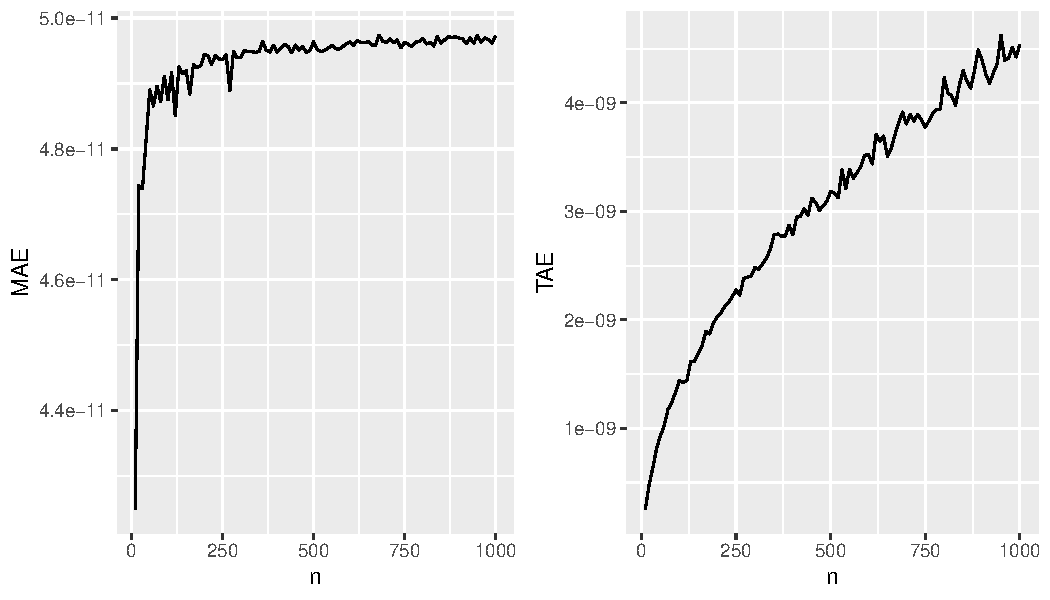
\includegraphics[width=0.8\textwidth]{figures/binom.pdf}
	\caption{ As $n$ increasing to 1000, the MAE is around $10^{-11}$ and the TAE is around $10^{-9}$}
	\label{fig: dft accuracy}
\end{figure}

From Figure 1, one can tell $\dft$ is reliable. The error is well controlled and smaller than $10^{-9}$ generally. The possible source of error is the machine error from inside of the C++ interface of Multi-Dimensional Fast Fourier Transformation algorithm. As dimension increases, the Fast Fourier transformation algorithm become imprecise. This is also the why compare with the result from \citeN{hong2013computing} our algorithm is less accurate. Figure 2 shows us similar results when the Binomial is replaced by Poisson Binomial, the error is small and due to FFT algorithm itself. Overall, it suffices to conclude that our $\dft$ algorithm is accurate and it can be used to compute true pmf.  

\begin{figure}[h]
	\centering
	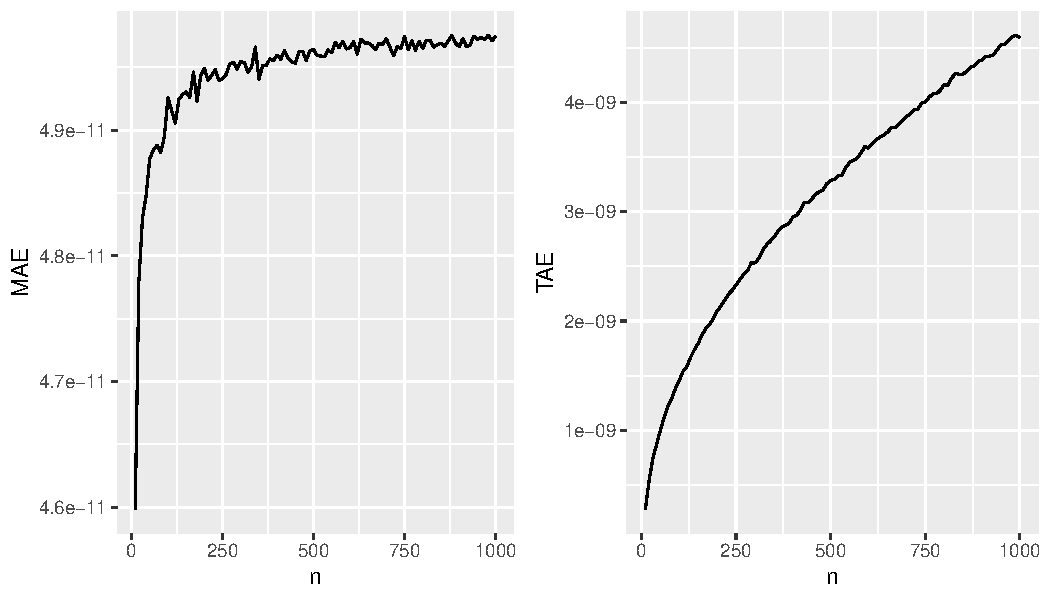
\includegraphics[width=0.8\textwidth]{figures/poib.pdf}
	\caption{Accuracy result of $\dft$ under Poisson Binomial senario}
	\label{fig: dft accuracy}
\end{figure}







\subsection{Accuracy of Normal Approximation and Simulation Method}
%%%%%%%%%%%%%%%%%%%%%%%%%%%%%%%%%%%%%%%%%%%%%%%%%%%%%%%%%%%%%%%%%%%%%%%%%%%%%%%%%%%%%%%%%%%%%%%%%
Among the three computing algorithms we proposed, one of them is able to calculate the exact probability while the other two are approximation methods. Therefore, it is necessary to explore accuracy of the approximation methods under different circumstances. The accuracy metric for $\NA$ is $\MAE$. For $\SIM$ we only consider the maximum probability and probability mass points of 0.95, 0.90 quantiles due to computation capability of device. Probability mass points computed by $\dft$ are considered as true probabilities, denote it as $p_{\rm true}$.
$\MAE$ and $\TAE$ for normal approximation are given by
\begin{equation*}
    \MAE = \max_{\xvec \in \chi}|p_{\NA}(\xvec)-p_{\rm true}(\xvec)|,
\end{equation*}
For simulation method the error metric is given via the difference between the selected probability mass points(maximum, 0.95 and 0.90 quantiles) calculated by $\SIM$ and $\dft$. 

For fixed $n$ from 1 to 75 and $m=3$, randomly generate 5000 $\Pmat$s to exclude the noise effect followed by calculating error metrics with respect to each methods. The results are shown via Figure 3 and Figure 4. In Figure 3, we mainly study the relationship between accuracy and simulation times $\mbox{B}$. The top lines in three plots are of $B=10$,  the middle lines are of $B=10^5$ and the rest are of $B=10^7$. Observe that the gap between lines reduces as $n$ increases possibly due to sparsity. The accuracy performance when $B$ is evidently better than when $B$ is small. We can tell from the plots that $B=10^7$ might be a good choice for user since it provide an accuracy error as small as $10^{-5}$.
\begin{figure}[h]
	\centering
	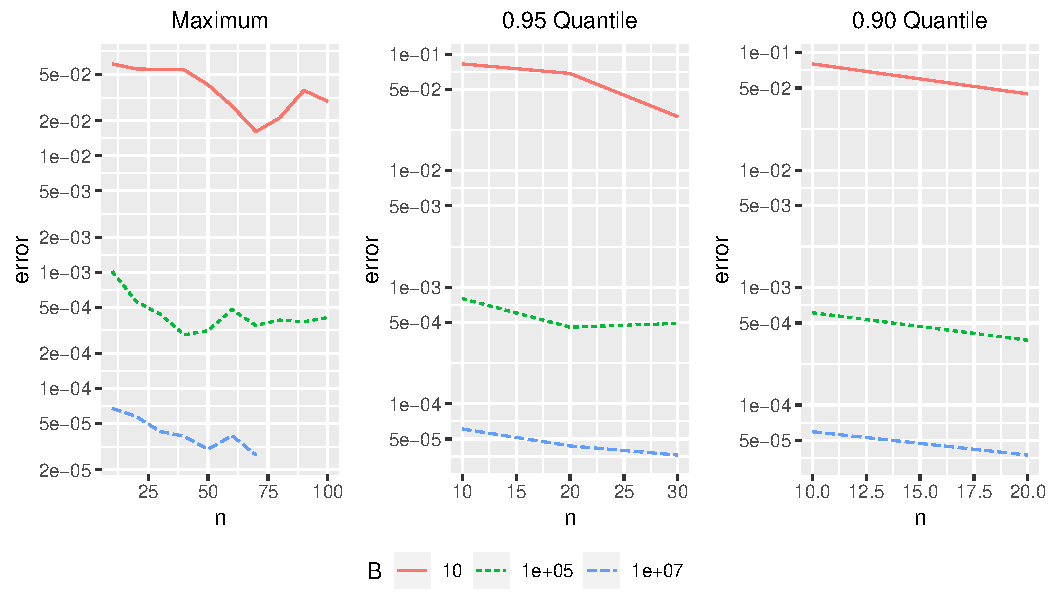
\includegraphics[width=0.8\textwidth]{figures/simulation.pdf}
	\caption{Accuracy of $\SIM$ method based on quantile of $\PMD$ when $m=3$}
	\label{fig: dft accuracy}
\end{figure}

Specifically, for $\NA$ we introduce a baseline called $\textbf{Original}$ to express the sparsity of $\PMD$ as $n$ and $m$ increase. The $\textbf{Original}$ is just to estimate all probability mass points by 0s. We can see through the plot the baseline is decreasing which is resulting from sparsity. From Figure 3, for given $m$, as $n$ increase the solid line which represent $\NA$ is always under the dashed baseline. The gap between the two lines grows wider as $n$ gets larger for fixed $m$ indicates that $\NA$ is more accurate when $n$ is large regardless of sparsity.
\begin{figure}[h]
	\centering
	\includegraphics[scale=0.8]{figures/mae.pdf}
	\caption{$\MAE$ of $\NA$ compared with baseline(Original)}
	\label{fig: dft accuracy}
\end{figure}



%%%%%%%%%%%%%%%%%%%%%%%%%%%%%%%%%%%%%%%%%%%%%%%%%%%%%%%%%%%%%%%%%%%%%%%%%%%%%%%%%%%%%%%%%%%%%%%%%
\subsection{Time Efficiency of DFT-CF method}
As a method to compute the whole pmf, we need to consider $\dft$'s time efficiency especially when the dimension is large. The method actually calculates $(n+1)^{m-1}$ probability mass points that includes the possible outcomes of $\PMD$ which is $\binom{n+m-1}{m-1}$. Because it takes every $x_j,j=1,\dots,m-1$ from 0 to $n$. The number $(n+1)^{m-1}$ increases drastically as $m$ gets larger. When $m$ is small, the result is showed by Figure 5. When $m$ is moderate ($8 \leq m \leq 20$) or larger, using $\dft$ can be problematic since $(n+1)^{m-1}$ can be enormous such that the device either takes too long to compute nor unable to compute due to exhausted usage of RAM. 

We use the same device as for accuracy study to test the time efficiency of $\dft$. Figure 5 plots the average computing time of 1000 randomly generated $\Pmat$s using $\dft$. The scale of time is second(s) and the computing is done on the same device as for the accuracy study. The following plot (Figure 5) shows that the when $m$ is small (less or equal to 4), it is good to use $\dft$ to calculate the entire pmf. As we can see through the plot the computing time for $n=60, m=4$ is 16 seconds which is affordable. Even when $m=5$ and $n=40$ the time is around 100 seconds which is still acceptable. However, when $m=6$ or higher, increasing $n$ can make the computing time huge.
\begin{figure}[h]
	\centering
	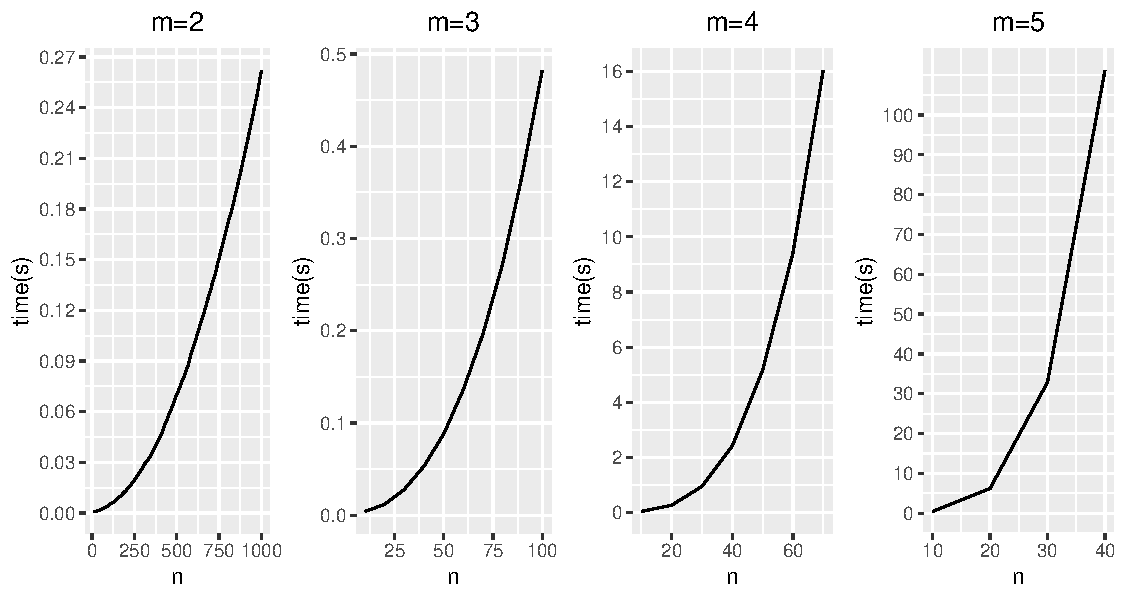
\includegraphics[scale=0.7]{figures/effi.pdf}
	\caption{Time efficiency study of $\dft$}
	\label{fig: dft efficiency}
\end{figure}


%%%%%%%%%%%%%%%%%%%%%%%%%%%%%%%%%%%%%%%%%%%%%%%%%%%%%%%%%%%%%%%%%%%%%%%%%%%%%%%%%%%%%%%%%%%%%%%%%
\subsection{Recommendations}
%%%%%%%%%%%%%%%%%%%%%%%%%%%%%%%%%%%%%%%%%%%%%%%%%%%%%%%%%%%%%%%%%%%%%%%%%%%%%%%%%%%%%%%%%%%%%%%%%
According to the results of accuracy and efficiency study. We hereby give out our recommendations of which method to choose under what circumstances. For small $m$ and moderate $n$, the $\dft$ can be used. Since the computing time is affordable and the method is an exact method that can compute the entire pmf automatically. However when $m$ is moderate or large, this method can be very time consuming and will need a huge RAM. Thus for moderate $m$ ($5 \leq m \leq 20$) and small $n$, we encourage users to use simulation method with $B$ around $10^6$ to calculate partial pmf that is of users' interests. By this way the accuracy will be maintained at a satisfied level and computing time will be affordable. For large $n$ including when $m$ is also large, the $\NA$ is recommended because the accuracy is backed up by central limit theory. If only calculate partial pmf, computing time will not be a concern.

%%%%%%%%%%%%%%%%%%%%%%%%%%%%%%%%%%%%%%%%%%%%%%%%%%%%%%%%%%%%%%%%%%%%%%%%%%%%%%%%%%%%%%
\section{Applications}
%%%%%%%%%%%%%%%%%%%%%%%%%%%%%%%%%%%%%%%%%%%%%%%%%%%%%%%%%%%%%%%%%%%%%%%%%%%%%%%%%%%%%%
\subsection{Calculation of Voting Probability}

  In voting scenarios, people always pay attention to the election result. The most thing we usually care about is who will win the election and how many chances each candidate has to win the election. A Poisson Multinomial distribution can fit the situation perfectly under some assumptions.\\

Suppose a election has $n$ voters and $m$ candidates, there will be $N = \binom{n+m-1}{m-1}$ possible outcomes denoted as $\boldsymbol{x}_r, r = 1, \dots, N$, respectively. Each $\xvec_r$ is a 3 dimension vector that has three elements denoting the number of votes each candidate gets. Assume we know the $\Pmat$ based on prior polls, for example, we can always estimate the approval rate of each candidate in a certain constituency from the monthly polls or exit polls. Then we are able to compute the notional result.\\

To demonstrate that, suppose we have ten electoral voters and three candidates with $\Pmat$ matrix that has means of column one, two and three to be $0.3631,0.3405$ and $0.2964$, the first five rows are as following,
\begin{equation*}
    \Pmat[1:5,] = \begin{pmatrix}
0.071 & 0.589 & 0.340\\
0.365 & 0.195 & 0.440\\
0.445 & 0.505 & 0.050\\
0.353 & 0.382 & 0.265\\
0.620 & 0.111 & 0.269
    \end{pmatrix}
\end{equation*}
To compute the probability of each candidate winning the election, just need to introduce constraints. For instance, under the constraint $\chi_1 = \left\{\text{the first element is the largest one}\right\} = \left\{x_1>x_2, x_1>x_3; x_1, x_2,x_3 \in \left\{0,\dots,10\right\}\right\}$, we are able to compute the winning rate of the first candidate is
\begin{equation*}
    p(\text{the 1st candidate wins}) = \sum_{\boldsymbol{x} \in \chi_{1}} p(\boldsymbol{x}) = 0.3429
\end{equation*}
Similarly, the probabilities for the second candidate and the third candidate to win are $0.2745$ and $0.2001$. Additionally, the most possible result is $\boldsymbol{x} = (4,3,3)$, which has probability 0.08546.




%%%%%%%%%%%%%%%%%%%%%%%%%%%%%%%%%%%%%%%%%%%%%%%%%%%%%%%%%%%%%%%%%%%%%%%%%%%%%%%%%%%%%%
\subsection{Statistical Inference for Aggregated Data}\label{sec:model.est.inf}	
First introduce the "Logistic-like" model to fit a given aggregated dataset with selected features and a categorical response variable that has $m$ categories. 
By dividing the rows of our data into $H$ groups $G_1,\dots,G_{S}$ via some given criterion, the group size of each group is $s_i,i=1,\dots,S$. Each $s_i$ are positive integer but not necessarily equal to each other. Let the quantity for each category of group $G_i$ be $\boldsymbol{x}^{(i)} = (x_1^{(i)}, \dots, x_m^{(i)})'$, $m$ is the category number. Denote $\boldsymbol{H}^{(i)}$ to be the covariate matrix of $G_i$, then $\boldsymbol{H}^{(i)} = (\boldsymbol{1}, \boldsymbol{h}_{1}^{(i)},\dots,\boldsymbol{h}_{s_i}^{(i)})'$ is a $s_i \times v$ matrix with first column being $\boldsymbol{1}$, where $v$ equals to the number of covariates plus one. Let $\Pmat^{(i)} = (p_{jk}^{(i)})$ be the SPM for group $G_i$, $i = 1, \dots, S$, $j = 1,\dots ,s_i$ and $k = 1,\dots, m$. Let the probability of getting $\boldsymbol{x}^{(i)}$ for group $G_i$ be $p(\boldsymbol{x}^{(i)})$. The total log-likelihood for all groups can be computed as
\begin{equation*}
    \ell = \sum_{i=1}^{S}\ell_i = \sum_{i=1}^{S}\log p(\boldsymbol{x}^{(i)})
\end{equation*}
Where $p(\boldsymbol{x}^{(i)})$ can be computed via Poisson Multinomial distribution with SPM $\Pmat^{(i)}$.\\
Set category $m$ as baseline and use softmax function to form the $\Pmat^{(i)}$ for each group through parameter $\boldsymbol{\beta} = (\boldsymbol{\beta}_1, \dots, \boldsymbol{\beta}_{m-1})$ as
\begin{align*}
    p_{j k}^{(i)} = \frac{\exp{\left(\boldsymbol{h}_{j}^{(i)} \boldsymbol{\beta}_{k}\right)}}{1 + \sum_{k=1}^{m-1}\exp{\left( \boldsymbol{h}_{j}^{(i)} \boldsymbol{\beta}_{k} \right)}}
    \quad k \neq m \quad \text{and } \quad
    p_{i,m}^{(i)} = \frac{1}{1 + \sum_{k=1}^{m-1}\exp{\left( \boldsymbol{h}_{j}^{(i)} \boldsymbol{\beta}_{k} \right)}}
\end{align*}

Then we are able to estimate our parameters on the direction of minimizing total log-likelihood and finally get our estimate $\wh{\Pmat}^{(i)}$. \\
In the rest of this part, we apply the model to the dataset ``ai4i". The dataset ``ai4i" is a synthetic machine failure dataset that reflects real predictive maintenance data encountered in industry. The data consists of 10000 products(rows) and 14 features(columns) including Product type, Air temperature, Process temperature, Rotational speed and others.

For demonstration purpose, here we only use the first 1000 rows and Product type as response variable, Air temperature and Process temperature as covariates. The feature Product type is categorical and has three levels, ``M", ``L", ``H", we denote them as category 1, 2, 3 for simplicity. The number of products that fall in category 1, 2, and 3 are 285, 601, and 114. The other two features are continuous.


We randomly divide the dataset into 100 groups $G_1,\dots,G_{100}$, the smallest group has size of three rows and the largest one has 18 rows. Note that readers can use other criterion to divide the dataset by their own. Notice the covariate number is three including intercept and the response has three categories, thus the dimension of our parameter matrix $\boldsymbol{\beta}$ will be $3 \times 2$ if we set category 3 as baseline.

The estimates of the parameters are
\begin{equation*}
\wh{\boldsymbol{\beta}} =
\begin{pmatrix}
 1.07484986 & 2.2820922 \\
 1.62342045 & 1.9108976 \\
 -0.06277732 &-0.8455964
\end{pmatrix}
\end{equation*}
The corresponding $\wh{\Pmat}^{(1)}$ and $\wh{\Pmat}^{(5)}$ for group 1 and group 5 are
\begin{equation*}
    \wh{\Pmat}^{(1)} = \begin{pmatrix}

 0.11914 & 0.63310 & 0.24776\\
 0.12326 & 0.57268 & 0.30406\\
 0.14809 & 0.47560 & 0.37631\\
 0.14504 & 0.56971 & 0.28525\\
 0.12451 & 0.54095 & 0.33454\\
 0.04170 & 0.55944 & 0.39886\\
 0.03559 & 0.53568 & 0.42873\\
 0.04890 & 0.54668 & 0.40442
    \end{pmatrix}, \quad
    \wh{\Pmat}^{(5)} = \begin{pmatrix}
 0.15604 & 0.70766 & 0.13630\\
 0.14469 & 0.73976 & 0.11555\\
 0.11246 & 0.67372 & 0.21382\\
 0.12036 & 0.64885 & 0.23079\\
 0.11263 & 0.61304 & 0.27433\\
 0.11563 & 0.55029 & 0.33408\\
 0.11774 & 0.61672 & 0.26554\\
 0.15071 & 0.52510 & 0.32419\\
 0.13878 & 0.56645 & 0.29477\\
 0.08194 & 0.54561 & 0.37245\\
 0.06307 & 0.58191 & 0.35502
    \end{pmatrix}
\end{equation*}
For group 1 and 5, $\boldsymbol{x}^{(1)} = (1,5,2)'$ and $\boldsymbol{x}^{(5)} = (2,6,3)'$, so $p(\boldsymbol{x}^{(1)}) = 0.070$, $p(\boldsymbol{x}^{(5)}) = 0.067$.
%%%%%%%%%%%%%%%%%%%%%%%%%%%%%%%%%%%%%%%%%%%%%%%%%%%%%%%%%%%%%%%%%%%%%%%%%%%%%%%%%%%%%%

%%%%%%%%%%%%%%%%%%%%%%%%%%%%%%%%%%%%%%%%%%%%%%%%%%%%%%%%%%%%%%%%%%%%%%%%%%%%%%%%%%%%%%
\subsection{Uncertainty Quantification in Classification}
In machine learning classification problem with multiple labels, for each unit in the test set, the probability of the unit belongs to each class is computed. Usually, the predicted class is assigned as the highest probability. In the classifiers (i.e., soft classification), the unit class is randomly assigned according to the predicted probabilities, leading to randomness in the confusion matrix. The PMD can be used to characterize the distribution of the counts in the confusion matrix.


%
%Yueyao: reliability course project used EL images for classification. The confusion matrix is obtained (Table 4 of the course report). In some senses, Table 4 only provide the point estimates, with PMD the distribution of the counts in each cell can be found, and can be displayed by an array of histograms.

In this section, we consider an Electroluminescence (EL) image classification example to illustrate the usage of PMD in machine learning classification problems. In the photovoltaic (PV) reliability study, the EL image is an important data type that reveal information about the PV health status. Because disconnected parts do not irradiate, the darker areas in EL images indicate defective cells. The EL imaging provide visual inspection of solar panels and is a non-destructive technology for failure analysis of PV modules \shortcite{Deitsch2019}.

The work of \shortciteN{Deitsch2019},\shortciteN{Buerhop2018}, and \shortciteN{Deitsch2021} provide a public dataset of solar cells extracted from high resolution EI images of PV modules (\url{https://github.com/zae-bayern/elpv-dataset}). In total there are 2624 images. All images are preprocessed with respect to size and are eliminated distortion induced by the camera lens used to capture the EL images. Each image is manually labeled  with its degree of defectiveness. The degree of defectiveness is determined by two questions. The first is how do evaluators think the status of the solar cells, functional or defective; the second is how they are confident about their assessments. In total there are four labels as shown in Table \ref{tbl:el.label} and we marked them as Class A-D.

\begin{table}[h!]
	\centering
	\caption{Partitioning of solar cells into functional and defective, with an additional self-assessment on the rater's confidence after visual inspection. Non-confident decisions obtain a weight lower than 100\% for the evaluation of the classifier performance }
	\begin{tabular}{c|c|c|c|c}
		\hline
		\hline
		Condition  & Confident?  &  Label $p$ & Weight $w$ & Class \\
		\hline
		\multirow{2}{*}{functional} & \cmark & functional & 0\% & A\\
		& \xmark& defective  & 33\% & B\\
		\hline
		\multirow{2}{*}{defective} & \xmark & defective & 67\% & C\\
		& \cmark & defective & 100\%  &D\\
		\hline
		\hline
	\end{tabular}
	
	
	
	\label{tbl:el.label}
	
\end{table}
%According to the probability how likely the product is defective, we assign four labels to sollar cells, 0\%, 33.33\%, 66.66\%, 100\%.

We split our data to training data (80\%) and test data (20\%), then train a CNN model on the training set. In CNN model, we use Relu activation function and set the kernel size $3 \times 3$ and stride $1 \times 1$. For each image in the testing set, the model provides a probability that the prediction belongs to each class. Table~\ref{tbl:elpmat} provides a subset of the CNN model output. For true class for the first sample in Table~\ref{tbl:elpmat} is A. If we predict the class of the first sample using the highest probability, then the prediction is A and there's no randomness. If we allow the model to make predictions based on the probability vector as shown in the first row then there are randomness in the confusion matrix. We can consider the confusion matrix to follow a PMD distribution then we can quantify the uncertainty in confusion matrix using PMD.

Figure~\ref{fig:confusion.hist} shows the marginal probability of each cell. For example, in the first row first column panel cell in Figure~\ref{fig:confusion.hist}, we know the possible counts that the model correctly predict class A as well as the corresponding probability. In this way, we have a uncertainty quantification in the confusion matrix.


\begin{table}[ht]
\centering
\caption{An example of the probability vectors of a subset in testing set from the trained CNN model.}
\label{tbl:elpmat}
\begin{tabular}{rrrrr}
  \hline
 & A & B & C & D \\
  \hline
1 & 0.9230 & 0.0366 & 0.0107 & 0.0297 \\
  2 & 0.0736 & 0.0802 & 0.0513 & 0.7950 \\
  3 & 0.0000 & 0.0016 & 0.0006 & 0.9978 \\
  4 & 0.9170 & 0.0537 & 0.0062 & 0.0231 \\
  5 & 0.9579 & 0.0239 & 0.0070 & 0.0112 \\
  6 & 0.8991 & 0.0347 & 0.0132 & 0.0530 \\
   \hline
\end{tabular}
\end{table}


\begin{figure}
	\centering
	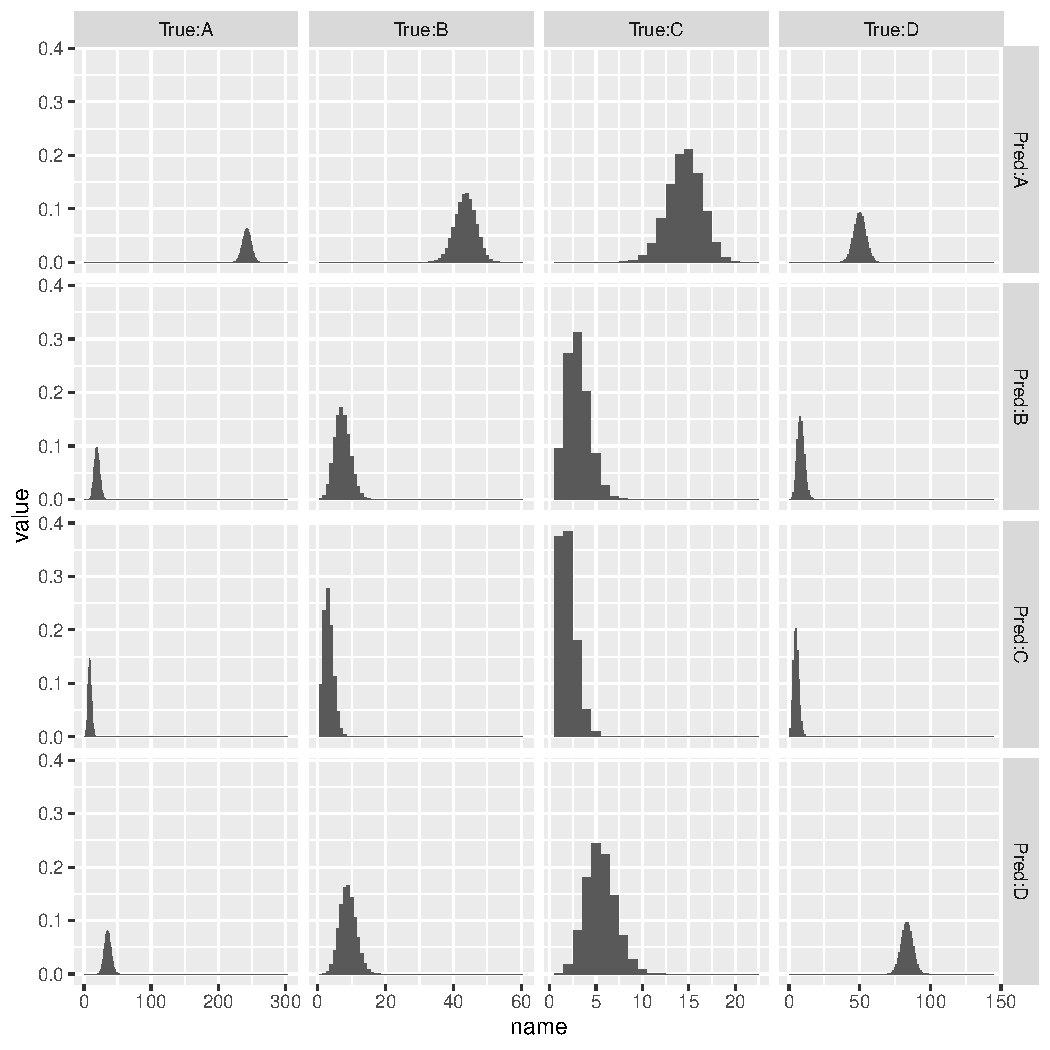
\includegraphics[width=0.9\textwidth]{figures/Confusionbar.pdf}
	\caption{The barplot shows the confusion matrix prediction. For each panel cell, the plot shows the corresponding prediction counts fall in this cell as well as their probability. We also present the mean and 95\% naive prediction interval.}
	\label{fig:confusion.hist}
\end{figure}
%%%%%%%%%%%%%%%%%%%%%%%%%%%%%%%%%%%%
\section{Illustrations of the R Package}
%%%%%%%%%%%%%%%%%%%%%%%%%%%%%%%%%%%%%%%%%%%%%%%%%%%%%%%%%%%%%%%%%%%%%%%%%%%%%%%%%%%%%%%%%%%%%%%%%
\subsection{Examples}
Illustrate the use of major functions in the R package.


%%%%%%%%%%%%%%%%%%%%%%%%%%%%%%%%%%%%%%%%%%%%%%%%%%%%%%%%%%%%%%%%%%%%%%%%%%%%%%%%%%%%%%%%%%%%%%%%%
\subsection{Benchmark of R Packages for Poisson Binomial Distribution}
%%%%%%%%%%%%%%%%%%%%%%%%%%%%%%%%%%%%%%%%%%%%%%%%%%%%%%%%%%%%%%%%%%%%%%%%%%%%%%%%%%%%%%%%%%%%%%%%%



%%%%%%%%%%%%%%%%%%%%%%%%%%%%%%%%%%%%%%%%%%%%%%%%%%%%%%%%%%%%%%%%%%%%%%%%%%%%%%%%%%%%%%%%%%%%%%%%%
\section{Conclusions and Areas for Future Research}
%%%%%%%%%%%%%%%%%%%%%%%%%%%%%%%%%%%%%%%%%%%%%%%%%%%%%%%%%%%%%%%%%%%%%%%%%%%%%%%%%%%%%%%%%%%%%%%%%

We develop algorithms that can be useful for computing the pmf of the PMD distribution, which is challenging to compute but useful in many application scenarios. We design three methods that are implemented in our algorithms. Among the methods, $\dft$ is an exact method, $\SIM$ is a simulation method and $\NA$ is a method using approximation theories. The accuracy and efficiency of the methods are guaranteed under given circumstances. We also recommend users to use $\dft$ when $m$ is small, use $\SIM$ when $m$ is moderate and $n$ is small, use $\NA$ when $n$ is large. However, there are still some fields remain to be explored. The computing speed of $\dft$ can be improved using more efficient Fourier transformation algorithms or we could find a way to calculate only the $\binom{n+m-1}{m-1}$ possible outcomes rather than $(n+1)^{m-1}$ probability mass points which contains a large amount of points have values equal to 0. $\SIM$ method is still time consuming although it can compute some cases that $\dft$ are unable to, once we develop more efficient exact algorithms, $\SIM$ could be replaced. Untill now, we are still unable to compute the pmf of $\PMD$ when $m$ is large, this area remains to be disclosed.



	
%%%%%%%%%%%%%%%%%%%%%%%%%%%%%%%%%%%%%%%%%%%%%%%%%%%%%%%%%%%%%%%%%%%%%%%%%%%%%%%%%%%%%%%%%%%%%%%%%%%%%%%%%%%%%%%%%%%%

%\section*{Acknowledgments}
%%%%%%%%%%%%%%%%%%%%%%%%%%%%%%%%%%%%%%%%%%%%%%%%%%%%%%%%%%%%%%%%%%%%%%%%%%%%%%%%%%%%%%%%%%%%%%%%%%%%%%%%%%%%%%%%%

%\bibliographystyle{apacite}


\bibliographystyle{chicago}
\bibliography{refs}	

\end{document}

%%%%%%%%%%%%%%%%%%%%%%%%%%%%%%%%%%%%%%%%%%%%%%%%%%%%%%%%%%%%%%%%%%%%%%%%%%%%%%%%%%%%%%%%%%%%%%%%%%%%%%%%%%%%%%%%%%%%%%%%%%%%%%%%%%%%%%%

